% book/index.tex —— 封面、目录与全书章节索引

% ---- 封面（使用原版封面图，tikz overlay 铺满整页）----
\begin{center}
\thispagestyle{empty}
\begin{tikzpicture}[remember picture, overlay, inner sep=0pt]
\node at (current page.center)
{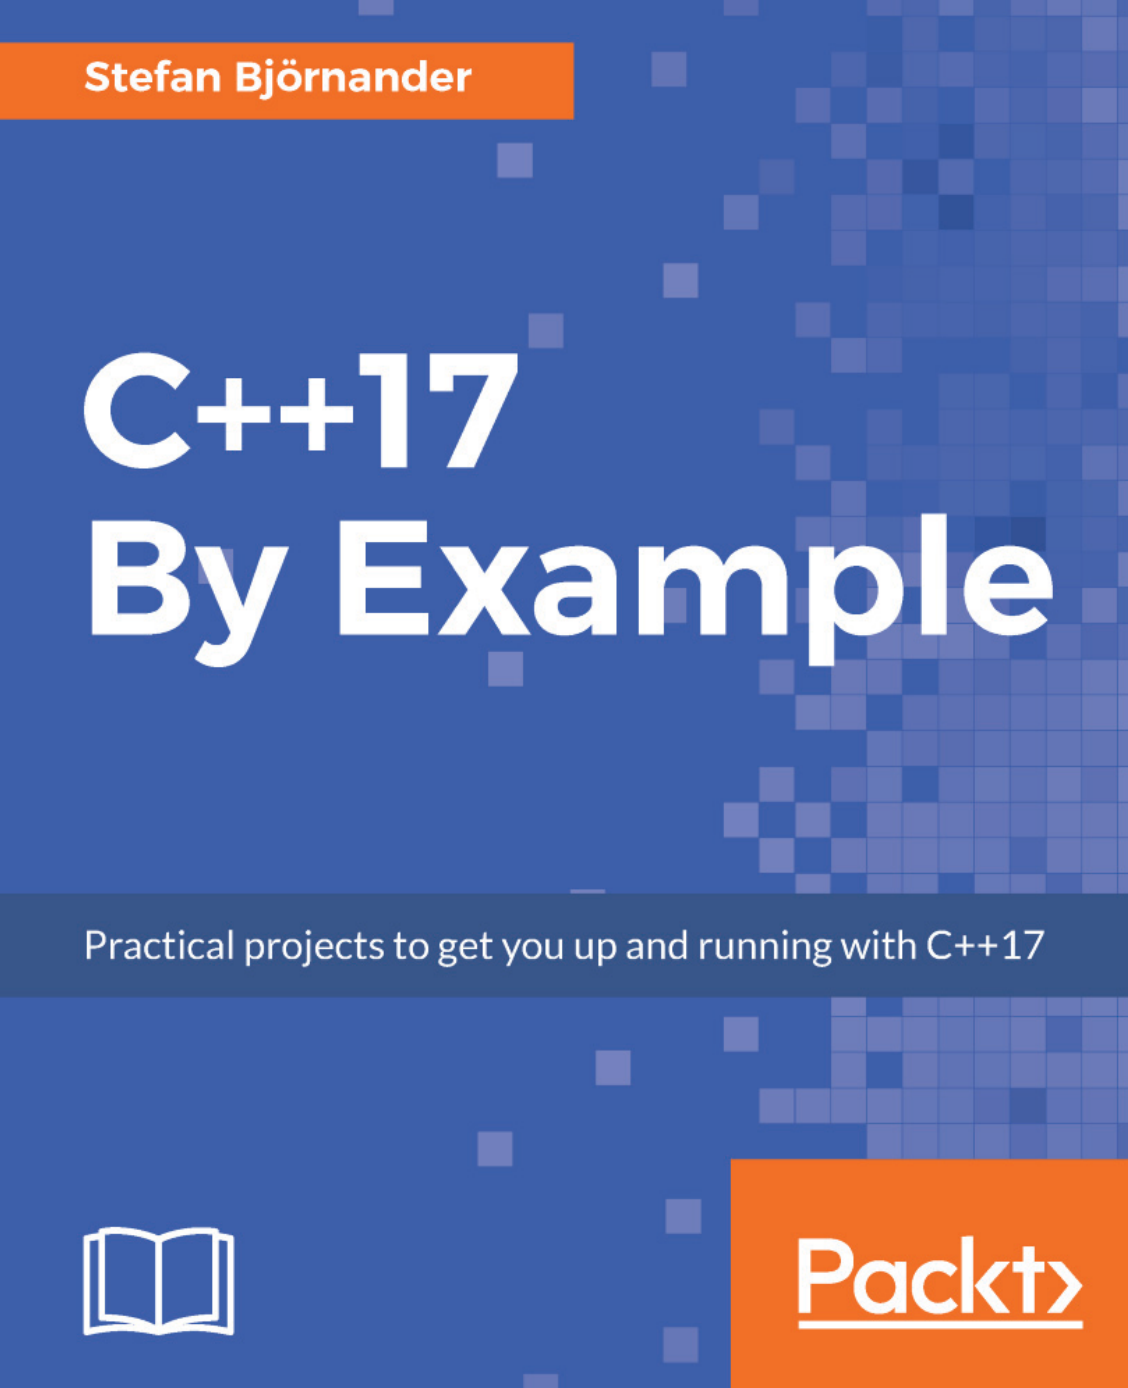
\includegraphics[width=\paperwidth,height=\paperheight,keepaspectratio]{images/cover.png}};
\end{tikzpicture}
\end{center}
\clearpage

% ---- 版权页 ----
\myFrontNoToc{content/front/copyright}

% ---- 献词 ----
\myFrontNoToc{content/front/dedication}

% ---- mapt.io / PacktPub.com（原书 page 5）----
\myFrontNoToc{content/front/mapt}

% ---- 贡献者（About the author / reviewer）----
\myFrontNoToc{content/front/about}

% ---- 目录（罗马页码）----
\tableofcontents
\clearpage

% ---- 前言类（正文前置页：阿拉伯页码自 1 起）----
\pagenumbering{arabic}
\myFront{前言}{content/front/preface}

% ---- 正文 10 章 ----
\myChapter{1}{初识 C++}{content/main/01}
\myChapter{2}{数据结构与算法}{content/main/02}
\myChapter{3}{构建图书馆管理系统}{content/main/03}
\myChapter{4}{基于指针的图书馆管理系统}{content/main/04}
\myChapter{5}{Qt 图形应用}{content/main/05}
\myChapter{6}{增强 Qt 图形应用}{content/main/06}
\myChapter{7}{游戏}{content/main/07}
\myChapter{8}{计算机对弈}{content/main/08}
\myChapter{9}{领域特定语言}{content/main/09}
\myChapter{10}{高级领域特定语言}{content/main/10}

% ---- 书末「其他你可能会喜欢的书籍」（原书 printed 414–416）----
\clearpage
\thispagestyle{empty}
\markboth{}{}
\addcontentsline{toc}{chapter}{其他你可能会喜欢的书籍}
\addtocontents{toc}{\protect\tocentryrule}
\vspace*{-32.8bp}
\begin{flushright}
  {\sffamily\fontsize{30bp}{34bp}\selectfont 其他你可能会喜欢的书籍\par}
\end{flushright}
\vspace{48.4bp}
\subfile{content/back/otherbooks}
\clearpage

% ---- 索引（标题与词条同页，两栏；首页无页眉页脚）----
\clearpage
\thispagestyle{empty}
\markboth{}{}
\addcontentsline{toc}{chapter}{索引}
\addtocontents{toc}{\protect\tocentryrule}
\vspace*{-32.8bp}
\begin{flushright}
  {\sffamily\fontsize{30bp}{34bp}\selectfont 索引\par}
\end{flushright}
\vspace{44bp}
\subfile{content/back/index}
